%&pdflatex

\documentclass[12pt]{article}

\usepackage[spanish, es-tabla]{babel}
\usepackage{enumerate}
\usepackage{lscape}
\usepackage{vmargin}
\usepackage{pdfpages}
\usepackage{fancyhdr}
\usepackage{graphicx}
\usepackage{float}
\usepackage{titlesec}
\usepackage[bottom]{footmisc}
\usepackage[hidelinks]{hyperref}
\usepackage{listings}
\usepackage{color}
\usepackage{colortbl}
\usepackage{xcolor}
\usepackage{amsmath}
\usepackage{array}
\usepackage{svg}
\usepackage{pgfgantt}
\usepackage[T1]{fontenc}
\usepackage[sfdefault]{AlegreyaSans} %% Option 'black' gives heavier bold face
%% The 'sfdefault' option to make the base font sans serif
\renewcommand*\oldstylenums[1]{{\AlegreyaSansOsF #1}}


%*******************************************************************************
\extrarowheight = -0.3ex
\renewcommand{\arraystretch}{2.25}
\setpapersize{A4}
\hypersetup{
    colorlinks=true,
    linkcolor=blue,
    urlcolor=purple,
    citecolor=black, 
    linktocpage=true,
}
\definecolor{gray95}{gray}{.95}
\definecolor{gray75}{gray}{.75}
\definecolor{barblue}{RGB}{153,204,254}
\definecolor{groupblue}{RGB}{51,102,254}
\definecolor{linkred}{RGB}{165,0,33}
\lstset{
    frame=Ltb,
    framerule=0pt,
     aboveskip=0.5cm,
     framextopmargin=3pt,
     framexbottommargin=3pt,
     framexleftmargin=0.4cm,
     framesep=0pt,
     rulesep=.4pt,
     backgroundcolor=\color{gray95},
     rulesepcolor=\color{cyan},
     %
     stringstyle=\ttfamily,
     showstringspaces = false,
     basicstyle=\small\ttfamily,
     commentstyle=\color{cyan},
     keywordstyle=\bfseries\color{purple},
     %
     numbers=left,
     numbersep=15pt,
     numberstyle=\small,
     numberfirstline = false,
     breaklines=true,
}

%minimizar fragmentado de listados
\lstnewenvironment{listing}[1][]
   {\lstset{#1}\pagebreak[0]}{\pagebreak[0]}


\lstdefinestyle{C}
   {
       language=C++,
   }

\lstdefinestyle{python}
    {
        language=Python,
    }

\setcounter{secnumdepth}{4}
%*******************************************************************************
%   Adding a new level of section --> subsubsubsection
%******************************************************************************
\titleclass{\subsubsubsection}{straight}[\subsection]

\newcounter{subsubsubsection}[subsubsection]
\renewcommand\thesubsubsubsection{\thesubsubsection.\arabic{subsubsubsection}}
\renewcommand\theparagraph{\thesubsubsubsection.\arabic{paragraph}} % optional; useful if paragraphs are to be numbered

\titleformat{\subsubsubsection}
  {\normalfont\normalsize\bfseries}{\thesubsubsubsection}{1em}{}
\titlespacing*{\subsubsubsection}
{0pt}{3.25ex plus 1ex minus .2ex}{1.5ex plus .2ex}

\makeatletter
\renewcommand\paragraph{\@startsection{paragraph}{5}{\z@}%
  {3.25ex \@plus1ex \@minus.2ex}%
  {-1em}%
  {\normalfont\normalsize\bfseries}}
\renewcommand\subparagraph{\@startsection{subparagraph}{6}{\parindent}%
  {3.25ex \@plus1ex \@minus .2ex}%
  {-1em}%
  {\normalfont\normalsize\bfseries}}
\def\toclevel@subsubsubsection{4}
\def\toclevel@paragraph{5}
\def\toclevel@paragraph{6}
\def\l@subsubsubsection{\@dottedtocline{4}{7em}{4em}}
\def\l@paragraph{\@dottedtocline{5}{10em}{5em}}
\def\l@subparagraph{\@dottedtocline{6}{14em}{6em}}
\makeatother

\setcounter{secnumdepth}{4}
\setcounter{tocdepth}{4}

%*****************************************************************************

\begin{document}

  \begin{titlepage}
    \centering
   {\bfseries\Large Universidad Carlos III de Madrid \par}
    \vspace{5cm}
    {\scshape\Huge Informe del Trabajo de Evaluación del Bloque 1 \par}
    \vspace{2cm}
    {\itshape\Large Diseño de circuitos electrónicos para comunicaciones}
    \vfill
    {\Large Autores: \par}
    \vspace{1cm}
    {\Large Markel Serrano y Daniel Theran}
    \vfill
    {\Large 11 de Octubre del 2022 \par}
  \end{titlepage}

  \section*{Apartado 1}

    \paragraph*{}
    En este apartado se pedía diseñar un filtro paso bajo en \textbf{Matlab} de forma que contase con un polo en la frecuencia de 30KHz.
    Para ello, es necesario utilizar la función "tf", que calcula la función de transferencia en tiempo continuo (H(s)).
    Después, transformamos esta función en H(z) mediante el uso del comando "c2d", que nos calcula la transformada Z de la función anterior.
    De esta forma, el código para generar las anteriores funciones, así como las variables necesarias y su correspondiente salida:

    \begin{figure}[H]
      \centering
      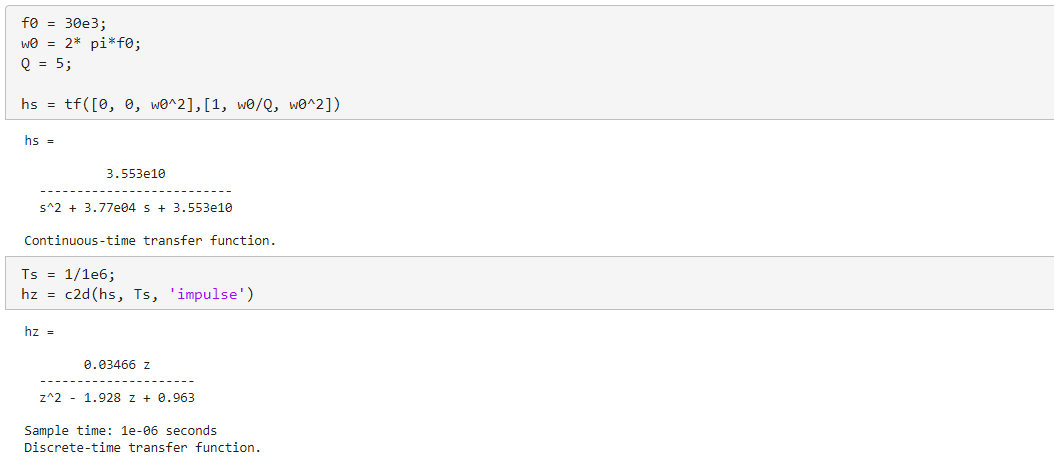
\includegraphics[width=1\linewidth]{Img/img_apartado_1.PNG}
      \caption{Entrada y salida del apartado 1 en Matlab}%
      \label{fig:img1}
  \end{figure}

    %%si quieres, tras esto se puede explicar un poco el significado de la función Hz, aunque tampoco le veo mucho sentido. Igual es mejor explicarlo en el apartado siguiente

  \section*{Apartado 2}
  
    \paragraph*{}
    En el segundo apartado se pide representar gráficamente ambas funciones. Para conseguir este objetivo se emplea la función "bode".
    De esta forma, la representación de la función de transferencia, tanto en tiempo continuo como en discreto, queda de la siguiente manera:

    \begin{figure}[H]
      \centering
      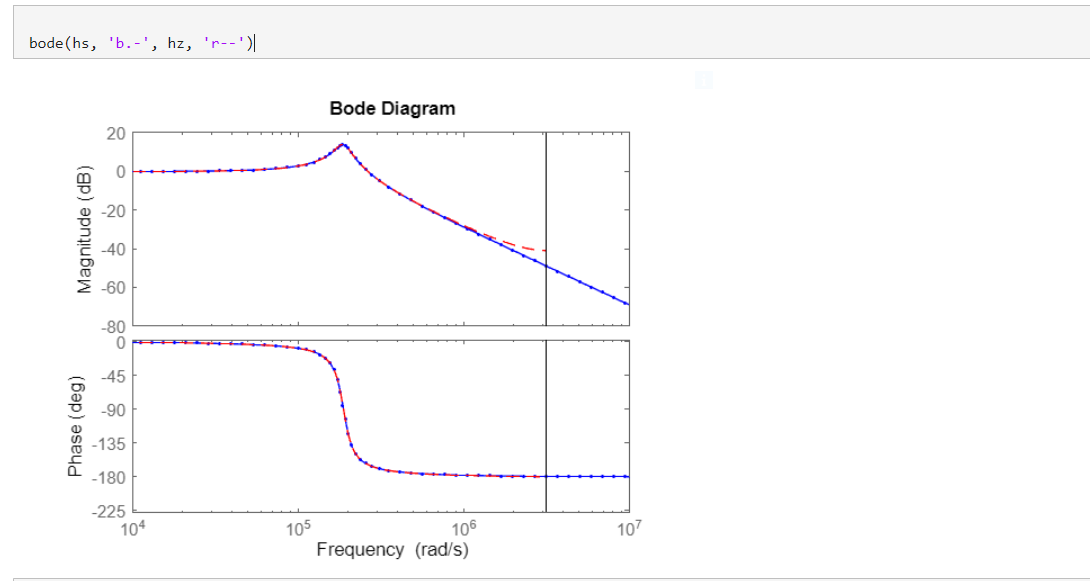
\includegraphics[width=1\linewidth]{Img/img_apartado_2.PNG}
      \caption{H(s) y H(z) representados en Matlab}%
      \label{fig:img2}
  \end{figure}

  \paragraph*{}
  Como se puede ver,

  %%falta tirarnos el moco con alguna explicación técnica
  
  \section*{Apartado 3}
  \section*{Apartado 4}
  \section*{Apartado 5}
  \section*{Apartado 6}
  \section*{Apartado 7}

  \paragraph*{}
  Para calcular valores de los condensadores tales que hagan al circuito diseñado comportarse como el circuito teórico del primer apartado,
  sus funciones de transferencia deben ser equivalentes. Para ello, se iguala término a término la función de transferencia teórica obtenida en el primer apartado
  con la función de transferencia calculada en el apartado 5, una vez se ha normalizado el término cuadrático de ambas funciones. Además, debemos suponer que los valores de C2 y C5 son iguales, e iguales a 20pF,
  y C1 y C4 son a su vez iguales.

  %%me parecía redundante meter aquí la expresión completa de las funciones cuando ya están en el apartado 1 y 5
  \paragraph*{}
  De esta forma, encontramos las siguientes equivalencias:
  
  \begin{itemize}
    \item $\frac{C_2}{C_2 + C_7} = 0.963$ 
    \item $\frac{C_1 \cdot C_4 }{C_5(C_2+C_7)} = 0.03466$
    \item $\frac{C_4\cdot C_3 - C_5 \cdot C_7 - 2 \cdot C_5 \cdot C_2}{C_5(C_2 + C_7)} = -1.928$
   \end{itemize}

   \paragraph*{}
   Despejando de las anteriores equivalencias, se obtienen los siguientes valores para los condensadores del circuito:

  \begin{itemize}
     \item $C_2 = C_5 = 20pF$
     \item $C_1 = C_4 = 3.79pF$
     \item $C_7 = 0.77 pF$
     \item $C_3 = 3.82pF$
   \end{itemize}


 \section*{Apartado 8}
 \section*{Apartado 9}
 \newpage
 \section*{Anexos: }
 \subsection*{Anexo I: Desarrollo de la función de transferencia de la primera etapa del filtro completo}
 \subsection*{Anexo II: Desarrollo de la función de transferencia del filtro completo}
  \section*{Apartado 8}
  \section*{Apartado 9}
  \newpage
  \section*{Anexos: }
  \subsection*{Anexo I: Desarrollo de la función de transferencia de la primera etapa del filtro completo}
  \subsection*{Anexo II: Desarrollo de la función de transferencia del filtro completo}

\end{document}
